\documentclass[journal]{IEEEtran}

\usepackage{times}
\usepackage{epsfig}
\usepackage{graphicx}
\usepackage{amsmath}
\usepackage[psamsfonts]{amssymb}
\usepackage{url}
\usepackage[pagebackref=true,breaklinks=true,letterpaper=true,colorlinks,bookmarks=false]{hyperref}

\begin{document}

\title{Surface EMG for Force Control of\\Mechanical Hands}

\author{Claudio~Castellini, Patrick van der Smagt, Giulio~Sandini
\thanks{C. Castellini \emph{(corresponding author)}
  is with the LIRA-Lab, University of Genova,
  viale F. Causa, 13, 16145 Genova, Italy.
  e-mail: claudio.castellini@unige.it.}%
\thanks{P. van der Smagt is with the DLR, German Aerospace Center,
  Institute of Robotics and Mechatronics, Oberpfaffenhofen, Germany.
  e-mail: smagt@dlr.de.}%
\thanks{G. Sandini is with the Italian Institute of Technology,
  via Morego, 30, 16100 Genova, Italy.
  e-mail: giulio.sandini@iit.it.}%
}

\maketitle

\begin{abstract}
  The dexterity of active hand prosthetics is limited not only due
to the limited availability of dexterous prosthetic hands, but
mainly due to limitations in interfaces. How is an amputee
supposed to command the prosthesis what to do (i.e., how to grasp
an object) and with what force (i.e., holding a hammer or grasping
an egg)? So far, in literature, the most interesting results have
been achieved by applying machine learning to forearm surface
electromyography (EMG) to \emph{classify} finger movements; but
this approach lacks, in general, the possibility of quantitatively
determining the force applied during the grasping act.

In this paper we address the issue by applying machine learning to the
problem of \emph{regression} from the EMG signal to the force a human
subject is applying to a force sensor. A detailed comparative analysis
among three different machine learning approaches (Neural Networks,
Support Vector Machines and Locally Weighted Projection Regression)
reveals that the type of grasp can be reconstructed with an average
accuracy of $90\%$, and the applied force can be predicted with an
average error of $10\%$N, corresponding to about $5$N over a range of
$50$N. None of the tested approaches clearly outperforms the others,
which seems to indicate that machine learning as a whole is a viable
approach.
%
%Notwithstanding the well-known bad conditioning of the surface EMG
%signal then, this looks highly encouraging in applying machine
%learning to enable amputees gain a fine control over advanced
%prosthetic hands, also since a surface EMG setup can be cheaply and
%easily realised and it is totally non-invasive.

\end{abstract}

\begin{IEEEkeywords}
advanced prosthetics, machine learning, EMG, force control, mechanical hands
\end{IEEEkeywords}

\IEEEpeerreviewmaketitle

\section{Introduction}
\label{sec:introduction}
\section{Introduction/Motivation}
\label{sec:intro}

\dropcap{A}utomatic speech recognition (ASR) is the ability of a machine
to convert human speech, coded as an audio signal, into words.
Potential applications of ASR range from human-computer interfaces
to informatics for the disabled to data mining in large speech corpora.
Despite decades of research, state-of-the-art ASR
systems still need to be trained upon very large and heterogeneous data sets
to account for speech variability.
%, or upon a single speaker's speech in controlled conditions.
And nevertheless, human beings show an excellent ability
of understanding one another's speech, independently of the speaker, the
accent, the pitch and speed, noise, etc.

Recent neuroscientific
evidence indicates that the brain motor areas responsible for producing labial
and dental phonemes are also involved in their perception; D'Ausilio et al. \cite{dausilio}
show that in a discrimination task of /b/,/p/,/d/ and /t/, trans-cranial magnetic
stimulation of the lips and tongue \emph{motor areas} creates a bias in favor
of the \emph{perception} of labials, and similarly, stimulation of the tongue
favors dentals. This suggests that motor information may be paramount for
understanding speech in humans.

Inspired by these finding, in this paper we investigate whether the knowledge of speech production in humans 
integrated into an automatic phoneme classifier improves the identification in the acoustic dimension 
of the specific behaviors of the /b/,/p/,/d/ and /t/ plosive consonants.
 
In ASR, approaches that combine explicit speech production knowledge and audio features
have been proposed (see \cite{king} for a review) as alternatives 
to the classic approach  in which the complex acoustic effects of speech production variability 
(e.g., due to speaking rate) and coarticulation (the phenomenon by which the phonetic realization of a phoneme is affected by its phonemic context) are directly and implicitly modeled in the acoustic domain.

%Although conclusions on the actual utility of speech production knowledge are somehow contradictory

By limiting our investigation on the utility of motor information to the much simpler (than ASR) task of four consonants classification\footnote{Note that a recognition task requires both segmentation of speech into phones and their classification.} we are able to relax working assumptions and avoid technical difficulties that so far have hampered a satisfactory integration of motor information into ASR systems. 

Additionally, from previous work it is not feasible to properly identify which aspects of the recognition process benefit from motor information. For example, motor knowledge may improve the modeling (and so the identification) of coarticulation effects that are seen in the training data set, but not necessarily improve the recognition of phonemes in unseen contexts, i.e., it may not necessarily improve the generalization ability of the ASR system. On the other hand the experimental setup we have designed has the main goal of investigating whether motor information improves the generalization ability of a phoneme classifier.  

%Although the integration of speech production knowledge in an ASR system often brings some improvements, %it is commonly held that the potential of speech production knowledge is far from being exhaustively exploited.  

To this end, we have focused on the automatic version of
the problem tackled in D'Ausilio et al.'s work. For each consonant,
a corresponding typical phonetic motor invariant (MI) was
identified according to basic physiology of speech;
e.g., a fast, voiced opening (plosion) of the lips for /b/, and so on.
MIs were then used to semi-automatically segment the audio/motor data found in a
database of speech/motor trajectories recorded from $6$ subjects.

Subsequently, a simple regression method (namely, a feed-forward neural network) was employed
to build an Audio-Motor Map (AMM), which converts audio features of the isolated segment to
features of the related MI. On an abstract level, an AMM is a mathematical proxy of a mirror
structure \cite{umilta-01}, reconstructing the distal speaker's speech production act while
listening to the related piece of speech.

To test the approach, we have devised three experiments involving a 
classifier in the form of a Support Vector Machine \cite{BGV92}. We wanted to check whether
the use of MI-based features, either those recorded in the database (the ``real''
motor features) or the AMM-reconstructed ones (a more ecological scenario),
could improve the classifier's performance. Our results show that this is the case,
especially when the classifier is trained on incomplete data sets such as 
per-speaker (e.g., training on speakers $1,2,3$ and testing on $4$) and
per-coarticulation(e.g., training on /ba/, /be/, /bi/, /bo/ and testing on /bu/); or when noise is added,
in which case motor features significantly help classification, even when added to a
state-of-the-art set of audio features about $20$ times larger than that extracted
from the MIs.

\subsection{Related Work}

It is known since the Sixties \cite{liberman1} that the audio signal of speech
cannot be effectively segmented down to the level of the single phoneme,
especially as far as stop consonants such as bilabial plosives
are concerned; in particular, their representations in the audio domain are
radically different according to the phoneme which immediately follows.
It remains an open question then, how humans can
distinctly perceive a common phoneme, e.g.,/b/ in  /ba/ and /bi/, since they
apparently have access to the speaker's audio signal only.

The explanation put forward by the so-called motor theory of speech perception
(MTS, \cite{liberman2,galant}) is that, while perceiving sounds,
humans reconstruct \emph{phonetic gestures}, the physical acts of
producing the phonemes, as they were trained since birth to associate
articulatory gestures to the sounds they heard. 

Even ignoring the motor theory of speech perception the use of speech production knowledge is appealing in that the coupling of articulatory and audio streams allows for explicit models of the effects of speech production phenomena (e.g., coarticulation) on the acoustic domain. These effects cannot be precisely modeled (e.g., when the phoneme /a/ affects the phonetic realization of /b/ in /ba/?)  or modeled at all (e.g., what happens when I utter a /o/ with exaggeratedly open jaw?) when the phonemic stream is directly mapped onto the acoustic dimension as in the standard approach to ASR.  

Different solutions have been proposed to integrate speech production knowledge into an ASR system and different types of speech production information has been used, ranging from articulatory measurements (see \cite{zlokarnik,stephenson,wrench}, for example) to symbolic non-measured representations of articulatory gestures that "replicate" a (symbolic) phoneme into all its possible articulatory configurations\footnote{Articulatory configurations are configurations of the positions of the phonetic articulators} (see \cite{richardson, livescu}, for example).
 
   
%One possible reason why ASR is so difficult is then that
%machines have in general no access to the motor representation of the
%audio signal they are supposed to understand. We hypothesize that motor 
%information might help ASR, especially when tests on different speakers and different
%coarticulations are performed: for example, when training on subject $A$ and
%testing on subject $B$, or when training on pseudo-words such as /ba/, /bi/,
%/be/ and then testing for the presence of /b/ in /bo/, /bu/ or even /br/.

Although some studies have shown increased word recognition accuracy when including speech production knowledge in ASR, it is commonly held that the potential of speech production knowledge is far from being exhaustively exploited. Limits of current approaches include: the use of the phoneme as basic unit (as opposed to articulatory configuration, for example) which appears to be too "coarse", especially in the context of spontaneous spoken speech 
%where coarticulation effects are more frequent and marked
;and  the lack of a mechanism that accounts for the different importance of articulators in the realization of a given phoneme (e.g., in the generation of phoneme /b/ lips are critical, i.e., important, while tongue is non-critical).

The traditional approach in which the speech signal is segmented into phones, often referred to as "beads on a string" approach, poses problems to an accurate modeling of spontaneous speech where coarticulation phenomena such as phone deletion or assimilation (where a phone assimilates some articulatory gestures of the preceding/following phone), are frequent and not always predictable and call for finer-grained basic units (see \cite{ostendorf})). To partly make-up for such limitation we propose an alternative approach where, instead of segmenting the audio stream looking at audio features only and then observing the articulatory gestures within the identified phones, we give priority to the motor information in that speech is segmented by searching for phone-specific patterns of the (critical) articulatory gestures.

%Concerning the necessity of a phoneme dependent distinction between critical and non-critical articulators we do not 
%Traditionally (e.g., \cite{bourl,salvi}), the audio speech signal is segmented with a
%fixed-length Hamming window, usually 20ms. long. The resulting sequence
%is then analysed in the frequency or cepstral domain and the
%resulting coefficients are used as features for a classification system.
%One negative aspect of this approach is that it
%neglects the qualitative overall characteristics of the
%phoneme being uttered: depending on the speed of the speech, a consonant
%can have different lengths and, by using the above approach, global
%information about it is lost (see \cite{ostendorf}, where this approach is
%dubbed ``beads-on-a-string''). Nevertheless, as far as we know, there is
%so far no widely accepted alternative method for speech segmentation,
%if the audio signal is the only one available. One attempt, but not based
%upon articulatory data atl all, appears in \cite{bourlard}.


During recognition, articulatory gestures have to be recovered 
from audio information as audio is the only signal available.
Reconstruction of articulatory features has been attempted since a long
time, but in most cases it is not derived from articulatory \emph{data}
gathered from human subjects. One pioneeristic case is that of Papcun
et al. \cite{papcun} where the AMM is carried out by a Multilayer Perceptron.
Our procedure for building the AMM is deeply inspired by this work.
%By using a Multilayer Perceptron we implicitly assume that all articulators have the same importance and that the AMM is a %one-to-one mapping.   
%Papcun et al. \cite{papcun} observed that non-critical articulators have higher variance (in terms of position) than critical %articulators. 
The Multilayer Perceptron tries to carry out the best recovery of all articulatory gestures while more emphasis to the recovery of the gestures of the critical articulators should be given to the detriment of the non-critical articulators, which have higher variance (in terms of position, see \cite{papcun,rose}). Although we do not address this issue, the simple fact that we only consider two articulators alleviates a problem that would be otherwise far more relevant if all articulators were taken into account\footnote{The higher variance of the non-critical articulators is the main cause that makes AMM a one-to-many mapping: different articulatory configurations result in the same acoustic realization. Solutions to properly address this "ill-posed" nature of the AMM have been proposed by Richmond et al. \cite{richmond} and Toda et al. \cite{toda}. }.

%and subsequently Korin Richmond's work
%\cite{richmond2002,richmond2007} who have been able to reconstruct point-by-point
%the trajectories of articulators from the audio signal to a remarkably low
%error rate. The procedure for building the AMM is deeply inspired by their
%work.

Interestingly, the idea of using information about the mechanisms involved in the production of a human action to improve its classification/recognition (in a domain different from the production domain) has not only been applied in the context of speech recognition. For example Metta et al. \cite{metta-06} and Hinton \cite{hinton-2006} 
have shown that articulatory data can improve classification accuracy in automated hand action classification.

%TODO  
% Transferring the method to speech perception seems
% like a natural choice.


\subsection{Related Work}
\label{subsec:relatedwork}
Machine learning has already been used for hand posture classification
using the EMG signal, at least in \cite{dunlop,fukuda,smagt}. In the
last work, in particular, as many as $9$ different postures could be
classified to a remarkable degree of accuracy; it is deemed that this
was possible since the hand postures would correspond to isometric
muscular configurations, i.e., precise force configurations. The EMG
signal is known to be related to the \emph{force} a muscle is applying
(see, e.g., \cite{deluca}), therefore if one wants to reconstruct the
hand position one must resort to classification performed in
controlled force conditions. On the other hand, as far as we know,
nobody has ever attempted to build a map from the EMG to the force the
fingers apply --- rather than classification, a \emph{regression}
task.

Our online optimisation procedure is based upon the concept of
sparsification of a function, meaning that only a subset of the
samples in the training set are used to build an approximation to a
target function. This is required in an online setting, since there is
no guarantee that the flow of data potentially usable for training
will ever cease. Of the tested approaches, both Support Vector
Machines and Locally Weighted Projection Regression try and build a
sparse solution; but in all cases, also including Neural Networks,
there is so far no guarantee that the set of samples selected to build
the solution will stop growing as more and more data are used to
train. SVMs in particular are deemed to build sparse solutions (bsaed
upon support vectors, actually), but a recent result
\cite{Steinwart03} shows that, really, the number of support vectors
is proportional to the number of training samples. Therefore one
cannot expect to build an eventually stable solution of an online
problem.

Other ways of reducing the number of support vectors have been tried,
such as \cite{bmvc} in which sparseness is achieved without losing any
accuracy, or, e.g., \cite{LeeM01,KeerthiCDC06} where a subset of the
support vectors is heuristically selected andfewer support vectors are
traded for larger classification/regression errors. Indeed the idea of
sparsifying a solution is not new and has been used, e.g., in a
Bayesian framework \cite{figueiredo03adaptive}; as well, the
sparseness of solutions in the framework of Support Vector Machines
has been exploited and improved, e.g., with Relevance Vector Machines
\cite{tipping00relevance}.

\textbf{[[Patrick, will you say something here about dexterous
prostheses and their control?]]}



\textbf{[[Patrick?]}

\section{Materials and Methods}
\label{sec:m&ms}

In this Section we describe in detail the experiment we have
conducted, and the methods we have employed to gather the data, filter
and analyse them.

\subsection{Experimental Setup and Design}
\label{subsec:setup}
\begin{figure*}[!t] \centering
  \begin{tabular}{ccc}
    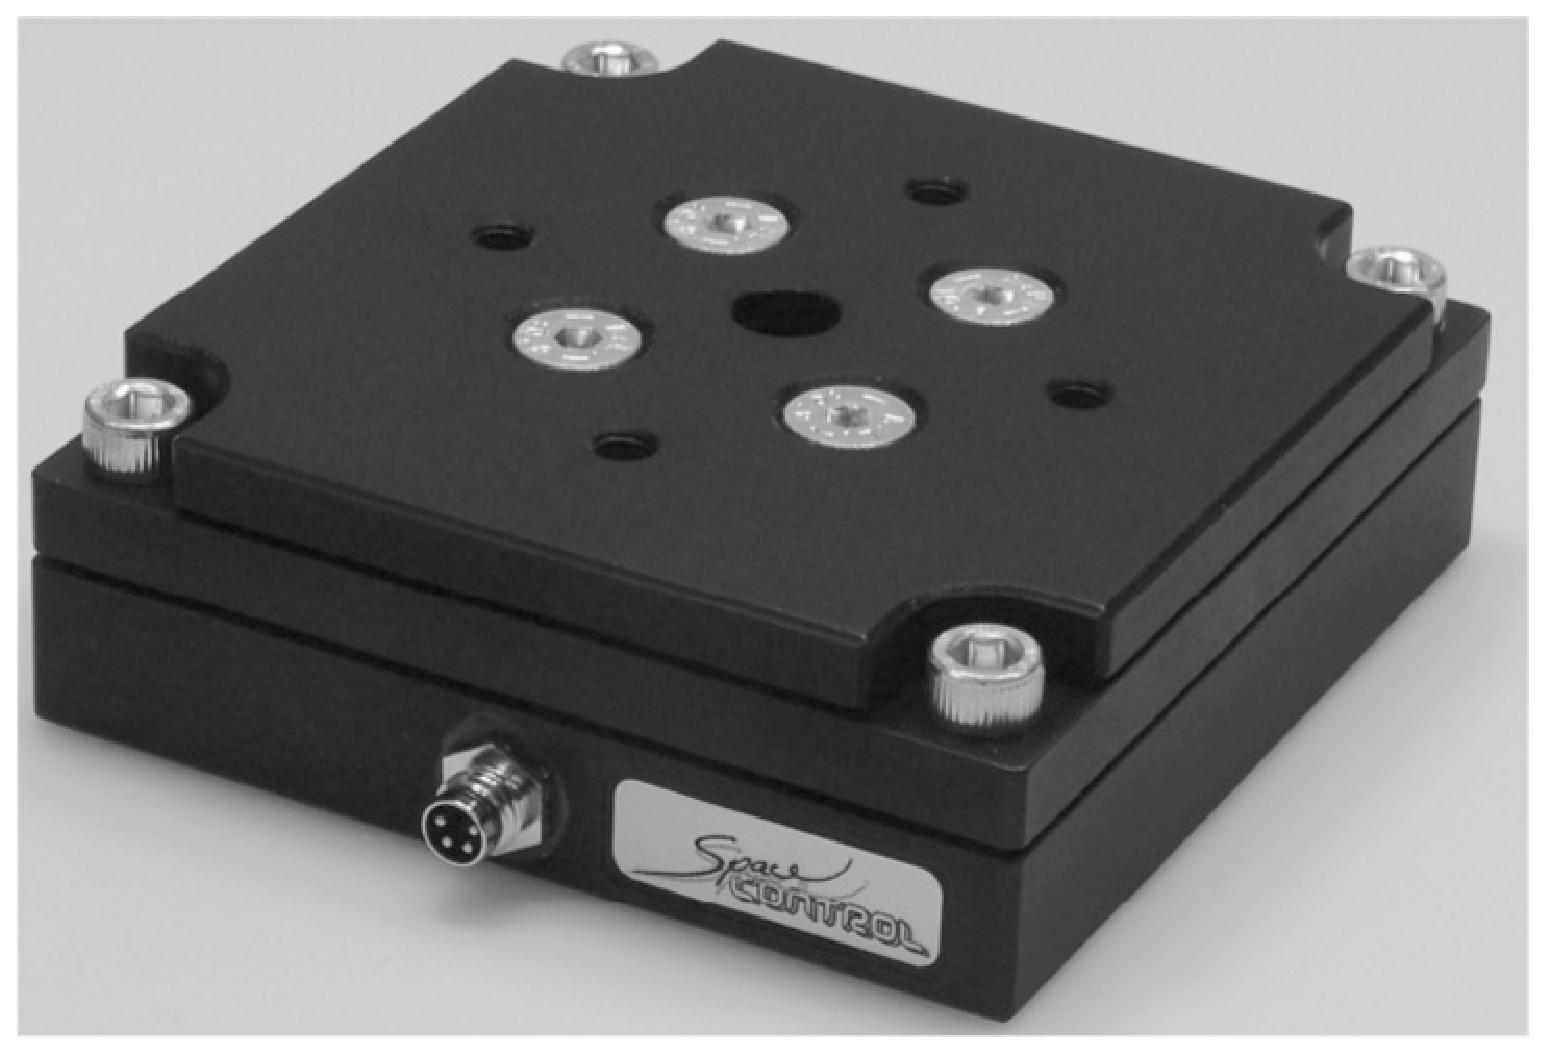
\includegraphics[height=0.16\textheight]{figs/OFTS} &
    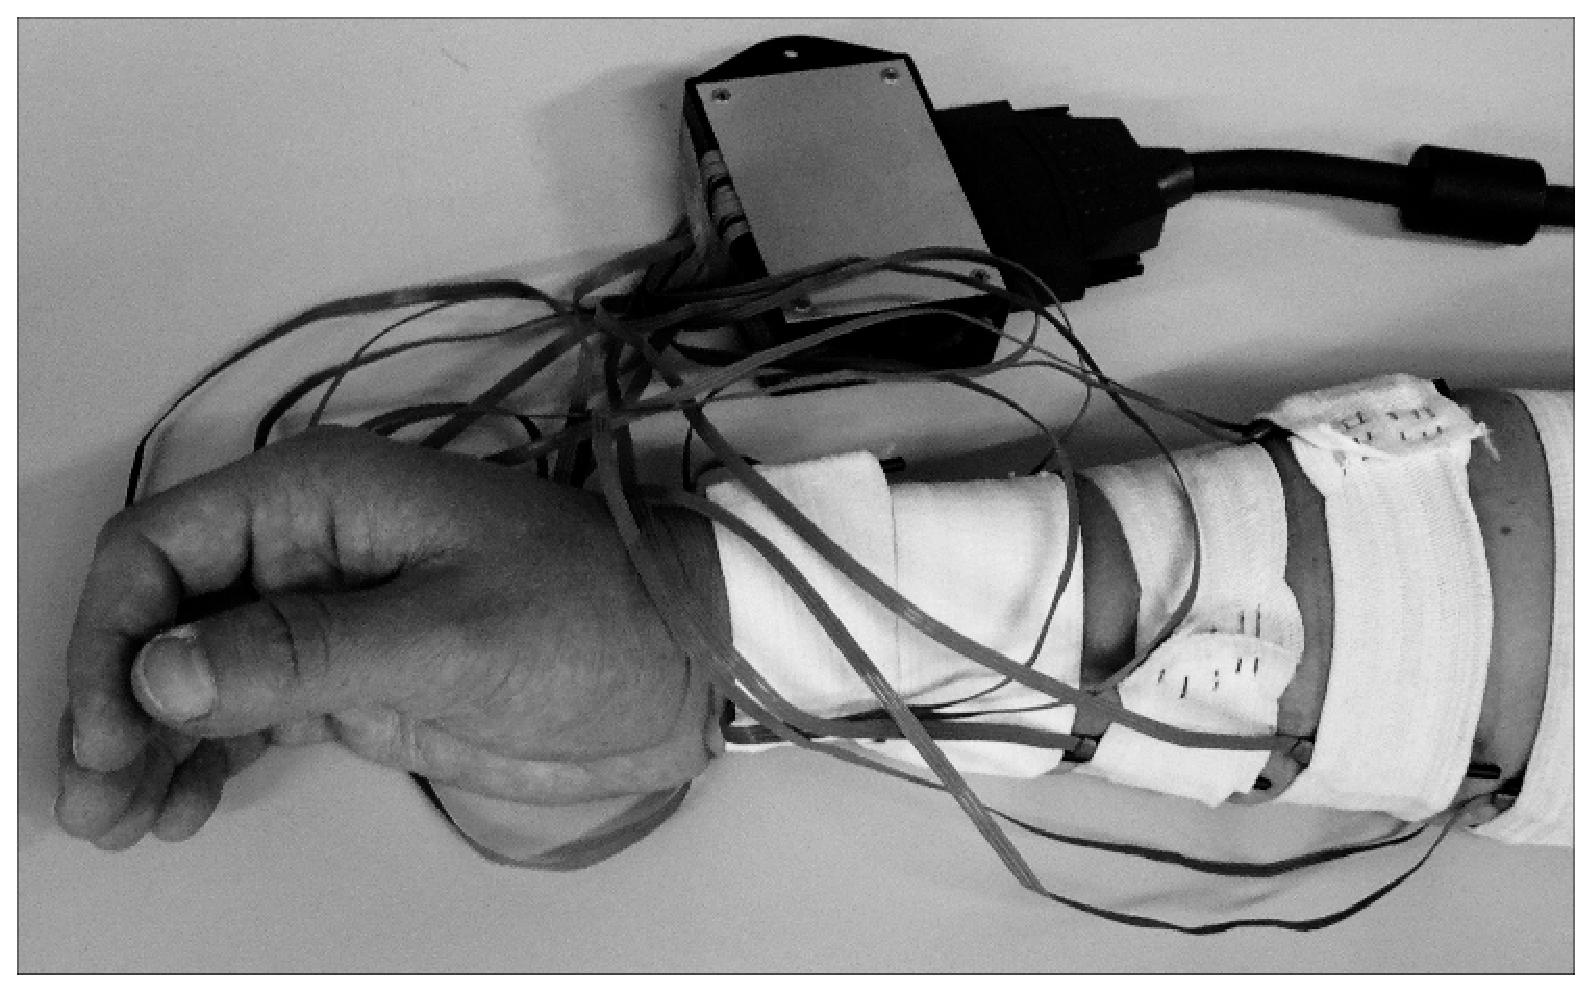
\includegraphics[height=0.16\textheight]{figs/setup} &
    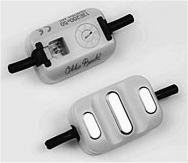
\includegraphics[height=0.16\textheight]{figs/ottobock} \\
    $(a)$ & $(b)$ & $(c)$ \\
  \end{tabular}
  \caption{The experimental setup. $(a)$ The SpaceControl OFTS
    force/torque sensor, large face up. $(b)$
    The arm of the subject with the EMG electrodes fitted and held in
    place by elastic bands. Electrode cables are wired in a box and
    then directed to a National Instruments PCI-6023E analogic/digital
    conversion card (not shown). $(c)$ An Otto Bock 13E200=50
    surface EMG electrode, with the amplification gauge (upper part of
    the Figure) and the three metallic contacts (lower part).}
  \label{fig:setup}
\end{figure*}

\subsubsection{General setup description}

The experiment consisted of freely, repeatedly grasping a SpaceControl
OFTS force/torque sensor \cite{ofts} orthogonally to its large face
(see Figure \ref{fig:setup} $(a)$). Four different ways of pressing
were allowed: opposing the thumb and index, the thumb and middle, the
thumb and ring or the thumb and all other fingers. The speed and force
was intentionally left to the subject's will. Four force sensing
resistors (FSRs) were applied on the subject's hand fingertips (thumb,
index, middle and ring), in order to be able to detect which grasp
type was used at each instant of time. At the same time, $10$ forearm
surface EMG electrodes were applied to the subject's forearm, held in
place by elastic bands, in order to gather information about the
muscle activation (see Figure \ref{fig:setup} $(b)$).

Numerical data from the EMG electrodes, FSRs and OFTS were gathered at
the fastest sampling rate we could obtain, that is, $256$Hz, using a
National Instruments DAQ PCI-6023E analogic/digital conversion card
\cite{nidaq}, mounted on a fast PC equipped with Windows XP.

\subsubsection{EMG signal and electrode placement}
\label{subsubsec:electrodes}

The $10$ EMG electrodes were applied to the subject's right forearm,
held in place by elastic bands. The electrodes were
double-differential Otto Bock 13E200=50 models (\cite{ottobock}, see
Figure \ref{fig:setup} $(c)$), each one gifted with an amplification
gauge ranging from $2000$ to $100000$ times. Initial qualitative
experiments revealed that a safe setting for the amplification gauge
was in the middle of the range, corresponding to about $14000$
times. This is in agreement with the EMG signal amplitude predicted in
the related literature (see, e.g., \cite{deluca}), that is about $100
\mu V$ on average: the voltages our DAQ card read ranged from $0V$ to
about $2.5V$.

Six of the electrodes were placed in pairs along the lower face of the
forearm, whereas four of them were applied in pairs on the upper
face. The initial positioning of the electrodes was chosen in order
for them to lie approximately on top of the muscles which elicit
finger movements; the precise placement was done following the
description in \cite{smagt}, which proved to be optimal for Support
Vector Machine classification of hand postures.

As far as the EMG signal is concerned, it must be remarked that it is
subject to remarkable changes depending on, at least, four orders of
factors:

\begin{enumerate}

  \item \emph{inter-subject variability.} All forearms are different
    from one another in shape, size and power.

  \item \emph{arm posture.} Besides finger movements and grasping, the
    forearm muscles are also involved in the motion of the arm. The
    EMG signal is therefore likely to change if the forearm is moved
    during signal acquisition, for example when switching from
    pronation to supination, or simply while walking around. Even
    raising the shoulder to lift the forearm from the table will
    result in remarkable signal changes.

  \item \emph{electrode displacement.} The intensity and quality of
    the EMG signal depends upon a correct placement of the electrode
    over a muscle. In principle, each electrode should be placed over
    a single muscle, precisely on top of the muscle belly, halfway the
    length of the muscle, and always exactly in the same place.
    Displacing the electrodes will alter the signal, and beside that,
    a precise placement is essentially impossible when dealing with
    surface forearm EMG.

  \item \emph{muscle fatigue.} As the muscles are used more and more,
    continually, fatigue changes the RMS of the EMG signal, calling
    for continual adaptation, at least over a reasonable set of
    different fatigue conditions.

\end{enumerate}

Problems $1$ and $2$ have been for now neglected by concentrating on
one subject only, male, aged $35$ and fully able-bodied, instructed to
keep the arm still and relaxed on a table in a confortable position,
with the palm orthogonal to the plane of the table. See the Discussion
Section for more about these issues.

As far as muscle fatigue and electrode displacement are concerned,
electrodes \emph{cannot} be expected to exactly lie in the very same
position every time the prosthesis is used; moreover, in a preliminary
round of experiments, muscle fatigue was clearly perceived by the
subject during the experiment. In this framework, the only possibility
to overcome these problems is to explicitly take them into account,
gathering enough data to be able to train the machine under different
conditions of electrode displacement and muscular fatigue.

We then organised the experiment as follows: the subject was
instructed to continually grasp the sensor over a period of time of
three to four minutes; then he was allowed to rest for about two
minutes. This was called a \emph{session}. It was expected that muscle
fatigue would appear already during one session. Three sessions were
gathered without taking the elastic bands off the subject's forearm,
in order \emph{not} to have electrode displacement within such a set
of sessions, that we called a \emph{group}. After each group, the
electrodes and bands were removed and the subject was allowed for a
much longer period of rest, ranging from half an hour to one
hour. During resting in-between groups, the subject could get back to
his normal muscular activity.

Five groups were then gathered during one day; and this procedure was
entirely repeated during another day. This procedure would allow us to
examine a relevant amount of data, gathered along a relatively long
period of time and under different conditions of muscle fatigue
(within one session) and electrode displacement (between groups). As
an example, Figure \ref{fig:drift}, pane $(a)$, shows the typical
electrode output during a session (moving average over about $10$
seconds). One can notice strong low-frequency components due to muscle
fatigue.

Spectral analysis of the EMG signal revelaed that all relevant
information is limited to $10$Hz (damping of $-30$dB at that
frequency), therefore sampling at $256$Hz proved to be a large
overshoot. We will employ this fact later on.

\begin{figure}[!ht] \centering
  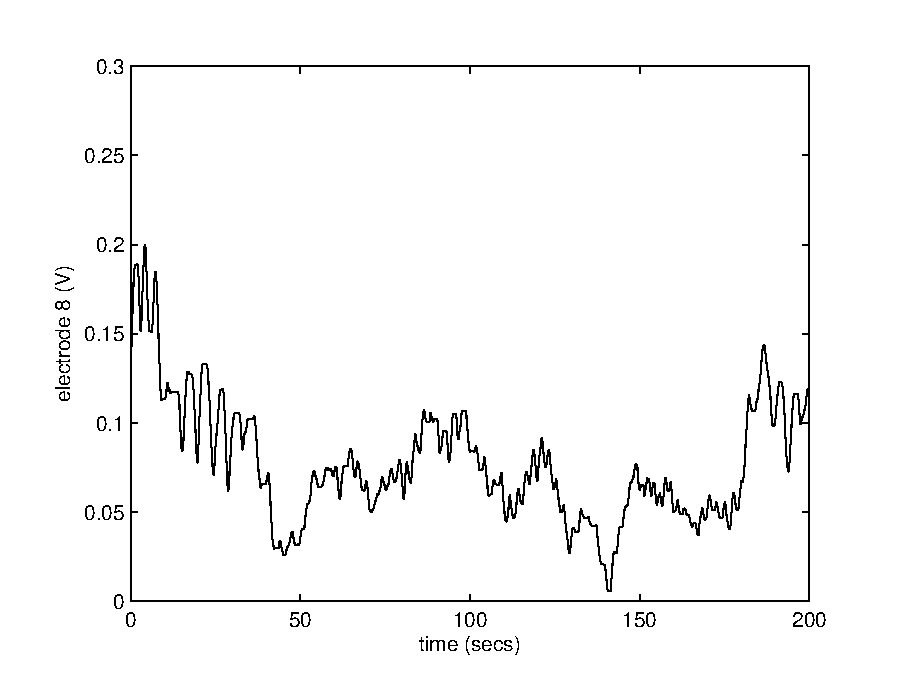
\includegraphics[width=0.45\textwidth]{figs/el8_movingAvg_s1}
  \caption{Typical behaviour of an electrode signal over a
    session (moving average over about $10$ seconds). Drifting can be
    clearly seen in the signal, due to muscle fatigue.}
  \label{fig:drift}
\end{figure}

\subsubsection{Force applied during the grasp}

The OFTS force/torque sensor would output a (negative) integer
numerical value ranging from $0$ to about $-5000$, expressed in
(negative) fiftieths of a Newton. After normalisation, the range of
the applied force would then be between $0N$ and $100N$, with a
resolution of $0.02N$. Linearity of the sensor is guaranteed, and was
anyway manually verified.

\subsubsection{Type of grasp}

The voltage values output by the $4$ FSRs applied onto the subject's
fingertips were monitored in order to understand which kind of grasp
the subject was applying to the sensor. A threshold was experimentally
decided, above which the finger would be defined \emph{in contact}
with the sensor. Using this technique, for each instant in time one of
five possible categories was established: $0$, no action; $1$, grasp
by opposing the thumb and index finger; $2$, opposing thumb and
middle; $3$ thumb and ring; and lastly $4$, grasp by opposing the
thumb and all other fingers.

It must be remarked here that the EMG signal would be altered
immediately at the onset of finger movement, which our setup was
unable to detect. This would result in potential wrong EMG values for
category $0$. Moreover, the FSRs have been experimentally determined
to suffer from a remarkable hysteresis effect, that is, they will
indicate slightly different voltage while pressing and releasing; this
is due to small rubber ends glued on top of the sensor surfaces, which
aid grasping by raising the static friction coefficient. Hysteresis is
also supposed to somehow degrade the quality of the learning. Because
of these factors we would never expected a close-to-$100\%$
classification accuracy, nor a perfect reconstruction of the applied
force. A better setup is currently being studied, which would avoid
these effects. Again, see the Discussion for more about this issue.


\subsection{Data Analysis}
\label{subsec:analysis}
The gathered data was analysed both for classification and
regression. \emph{Classification} is the process by which one wants to
assign a label to each sample in the input space, whereas in
\emph{regression} the target is a real-valued function of the values
of the input samples. Throughout this Section, we will assume that a
set of $l$ points in the input space is available, for which the
target (label or force value) is known; this set will be denoted by
$\{\xx_i,y_i\}_{i=1}^l$ and called \emph{training set}. As well, for
each experiment, a separate set of points, for which the targets are
not known, is assumed to be available, and this will be called the
\emph{testing set}. In general, the performance of a machine is tested
by training it on a training set and then testing it on a testing set,
possibly employing standard measures of the generalisation error, such
as cross-validation.

Taking into account the considerations of the previous Section, we set
the input space to be $\RR^{10}$, that is, one coordinate for each EMG
electrode; therefore, $\xx_i \in \RR^{10}, i=1,\ldots,l$. In the case
of classification, each category representing a grasping type would be
represented as an integer value, that is, $y_i \in \{0,\ldots,4\}
\subset \NN, i=1,\ldots,l$. In the case of regression, the force value
would be directly encoded as a real number, that is, $y_i \in \RR,
i=1,\ldots,l$. Before any analysis, all samples were normalised, as is
customary, by subtracting the mean values and dividing by the standard
deviation, for each input space dimension. No filtering whatsoever was
applied to the input signals, in order to have a more realistic,
delay-free result.

\subsubsection{Neural Networks}

Artificial Neural Networks (NNs or ANNs for short; see, e.g.,
\cite{bishop} for a comprehensive introduction) are probably the most
popular machine learning algorithm nowadays available for both
classification and regression. An ANN is a directed graph in which,
for every node, the weighted sum of the input values is evaluated;
this sum is then used as the argument of an \emph{activation function}
to determine the output of the node. The nodes fed the input values to
the network are called \emph{input layer}, and the nodes whose output
is taken as the output of the network are called \emph{output
layer}. Besides this, in general, an ANN can further have an arbitrary
number of nodes organised in \emph{hidden layers}, gifted with an
arbitrary edge topology.

An ANN is initialised with random weights; then, for every sample in
the training set, the network output is evaluated and its error with
respect to the target is considered. In order to reduce the error
then, a minimisation algorithm is then employed to change the weights
of the network, until the desired precision is reached. If the
generalisation error has been kept small, the network will then be
able to \emph{predict} the targets of the testing samples with a
reasonable accuracy.

For our experiment we strived to keep the ANN as simple as possible.
We then chose a basic feed-forward NN with $10$ units for the input
layer; one hidden layer with $10$ units with sigmoidal arcotangent
activation function; $5$ units in the output layer for classification,
each unit representing one category, and one unit in the output layer
for regression, the unit representing the target force value. The
network was trained via the \textbf{BOH} algorithm and learning
function \textbf{BOHBOH}; the mean-square error (MSE) was used as a
measure of performance. The training phase was stopped arbitrarily
after $30$ epochs. For each experiment, we repeated the training phase
$10$ times, in order to overcome the well-known problem of local
minima, and then gathered the best model found. No measure of
generalisation error was taken into account.

The network was implemented in Matlab, Windows version $7.1.0.246$
(R14) Service Pack 3, running on a bi-processor $1.8$GHz machine with
1GB on-board memory; we used the Matlab Neural Network Toolbox,
version $5.0.1$ (R2006b).

\subsubsection{Support Vector Machines}

Support Vector Machines (SVMs; see, e.g.,
\cite{BGV92,Burges98,Cristianini00}) are a machine learning method
able to determine the best candidate function for a classification or
regression problem, drawn from a functional space induced by the
choice of a binary function between points in the sample space,
$K(\xx_1,\xx_2)$, with $\xx_1, \xx_2 \in \RR^{10}$ in this case. $K$
is called \emph{kernel}. In the most general setting, the function
found is

\begin{equation} \label{eqn:sol}
  f(\xx) = \sum_{i=1}^l \alpha_i y_i K(\xx,\xx_i) + b
\end{equation}

\noindent where $b \in \RR$, whereas the $\alpha_i \in \RR$s are
Lagrangian coefficients obtained by solving a minimisation problem
whose cost functional is guaranteed to be convex. Because of this,
SVMs do not suffer from the problem of local minima; but their
training time is cubic in the number of samples in the training set,
as opposed to ANNs, for which it is \textbf{BOHBOH}.

In order to overcome this problem, which would have made our
experiment unfeasible, we have decided to use a \emph{uniformisation}
strategy on the training sets, before training the machines. The idea
is that, in a real-life set-up such as ours, there can be many input
samples located in the very same region of the input space, with very
similar target values. One obvious case is that of label $0$,
indicating no ongoing grasping: it is intuitively expected that a
large number of samples will be taken in that region of the input
space, since the subject will be in the $0$ condition for a longer
time than all other labels.

Since all functions involved in the experiment are due to human
motion, we can assume that they are continuous and, probably,
derivable up to any arbitrary order. Therefore it makes no sense for
an approach such as SVMs to sample the input space in a non-uniform
way such as that described above. The uniformisation procedure
consists of removing, from a training set, those samples which are too
close to each other, according to a suitable notion of inter-sample
distance.

In order to take into account the different variances of the EMG
electrode values, we have decided to adopt Mahalanobis's distance as
the inter-sample distance \cite{...}. Let $\xx_1, \xx_2 \in \RR^{10}$;
then the Mahalanobis distance between $\xx_1$ and $\xx_2$ is defined
as follows:

$$ MD(\xx_1,\xx_2) = \sqrt{(\xx_1-\xx_2)^T \Sigma^{-1} (\xx_1-\xx_2)} $$

\noindent where $\Sigma$ is the $10$x$10$ covariance matrix, evaluated
on the training set. $MD(\xx_1,\xx_2)$ is a distance in which each
summand is weighted inversely with respect to the variance of the
samples along that dimension of the input space: it is therefore a
measure of distance independent of the variance of the single
electrodes. Notice that if $\Sigma$ is replaced by the identity
matrix, $MD(\xx_1,\xx_2)$ is reduced to the usual notion of Euclidean
distance.

Since checking the inter-sample distance obviously takes a quadratic
time with respect to the number of samples, which was unfeasible, we
adopted an approximated method which was able to remove most, but not
all, samples with an insufficient Mahalanobis distance from any other
sample. After a few initial experiments we set the threshold distance
at $1$. All our experiments with SVMs were then performed on
uniformised training sets, using $5$-fold cross-validation and grid
search to find the optimal values of the standard Gaussian kernel
hyperparameters, $C$ and $\sigma$.

On the other hand, notice that no \emph{testing} set was uniformised,
since it would probably be unfeasible to apply the same procedure in
an on-line setting. Notice, further, that applying uniformisation
resulted in training sets which were considerably smaller than the
original ones, up to about $100$ times smaller.

Lastly, we employed a well-known freely available SVM package,
\emph{libsvm} v2.83 \cite{...}, in the Matlab wrapped flavour.

\subsubsection{Locally Weighted Projection Regression}

\textbf{LWPR - prendi qualcosa dalla rete. spiega gs e cv.}



\section{Experimental Evaluation}
\label{sec:exp}
We conducted two different experiments, one to predict the force measured
by the force sensor and another one to classify the grasp type.
The EMG data were the preprocessed as described in Section \ref{sec:preproc}.

As already mentioned in Section \ref{sec:adapt}, our working assumption is to have
 $N$ pre-trained models stored in memory.
Then new data comes from subject $N+1$ and the system starts
training, to build the $N+1$ model.
The performace is evaluated using unseen data from the subject
$N+1$.
To simulate this scenario and to have reliable estimation of the
performance, we used a leave-one-out approach: 
of the 10 subjects for which we have the data recordings, we train off-line
9 models. These will correspond to the $N$ stored models in memory. The data from the 10th 
remaining subject will be used for the adaptive learning of the $N+1$ model.
The training sequences are random subsets from the entire dataset, that is taken without
considering the order in which they were acquired.
This procedure is repeated 10 times, using in turns all the recorded subjects
for the adaptive learning of the model.

To assess the performance of the proposed adaptation method we compared it
to two baseline methods. The first one, that we call \emph{Prior}, consists in
using only the pre-trained models without updating them with the new training data.
Then we consider only the best performance of the 9 pre-trained models, to consider
the best-case scenario.
The second one, \emph{NoAdapt}, consists in using LS-SVM using only the new data
for training, as it would be in the standard scenario without adaption.
For classification we used the classification rate as a measure of
performance; for regression, the performance index is the correlation coefficient
evaluated between the predicted force signal and the real one. The
choice of the correlation coefficient, as opposed to the more standard
Mean-Square Error, is suggested by a practical consideration: when
driving a prosthesis, or even a non-prosthetic mechanical hand, we are
not interested in the absolute force values desired by the
user/subject, since mechanical hands usually cannot apply as much
force as human hands do, for obvious safety reasons\footnote{or, e.g.,
in teleoperation scenarios, they could be able to apply \emph{much
more} force than a human hand can.}. We are rather concerned about
getting a signal which is \emph{strongly correlated} with the
user/subject's will.
To build the  pre-trained models we used the standard SVM algorithm. All the parameters to be set during %of the
training ($C$ and $\gamma$ of the gaussian kernel) were chosen by cross-validation.

Figure \ref{fig:diff_cla} shows the average difference between 
the classification performance of \emph{NoAdapt} and our method. We see that using our adaptation
method there is always an improvement in performance, but when training is done on too little samples %are too
%few 
the standard deviations are big, i.e. depending on the subject there can be both a great gain or loss in performance. 
This is due to the high variance of the
leave-one-out error with few training samples. Still, the average gain is
almost $5\%$ when there are only 30 training samples and it seems to stabilize
around $1\%$ as the training samples increase.
Figure \ref{fig:cla_abs}.a shows the best performance obtained by our method
on a particular subject, while  Figure \ref{fig:cla_abs}.b shows the worst
performance achieved, of course on another subject. We see that in the best case the gain is quite significant,
while in the worst case we basically obtain  the performance of \emph{NoAdapt}. This last case is an example
where none of the models stored in memory matched the new distribution of the data, so the parameter
$\beta$ is automatically set to a very small value and in practice there is no transfer of prior knowledge. It is reasonable to think
that the performance of the method would increase with the number of stored
models, as it would increase the probability to find a good pre-trained model.
Note that in all the cases the performance of \emph{Prior} models, where well
below the performance of \emph{Adapt} and \emph{NoAdapt}: in Figure \ref{fig:cla_abs} is shown
only the performance of the best one among all the 9 stored models.
Similar observations can be done for the regression task in Figure \ref{fig:diff_reg}
and Figure \ref{fig:reg_abs}. In particular we gain in average 0.05 points on the score
of the correlation coefficient on the first 30 samples. Then the gain seems to decrease,
maybe approaching 0 when enough new training samples are acquired. However note that
the standard deviation bars are all above the zero, meaning that in worst case most of the time
we do not lose anything compared to the NoAdapt model (cf. Figure \ref{fig:reg_abs}.b).

\begin{figure}[t]
  \centering
  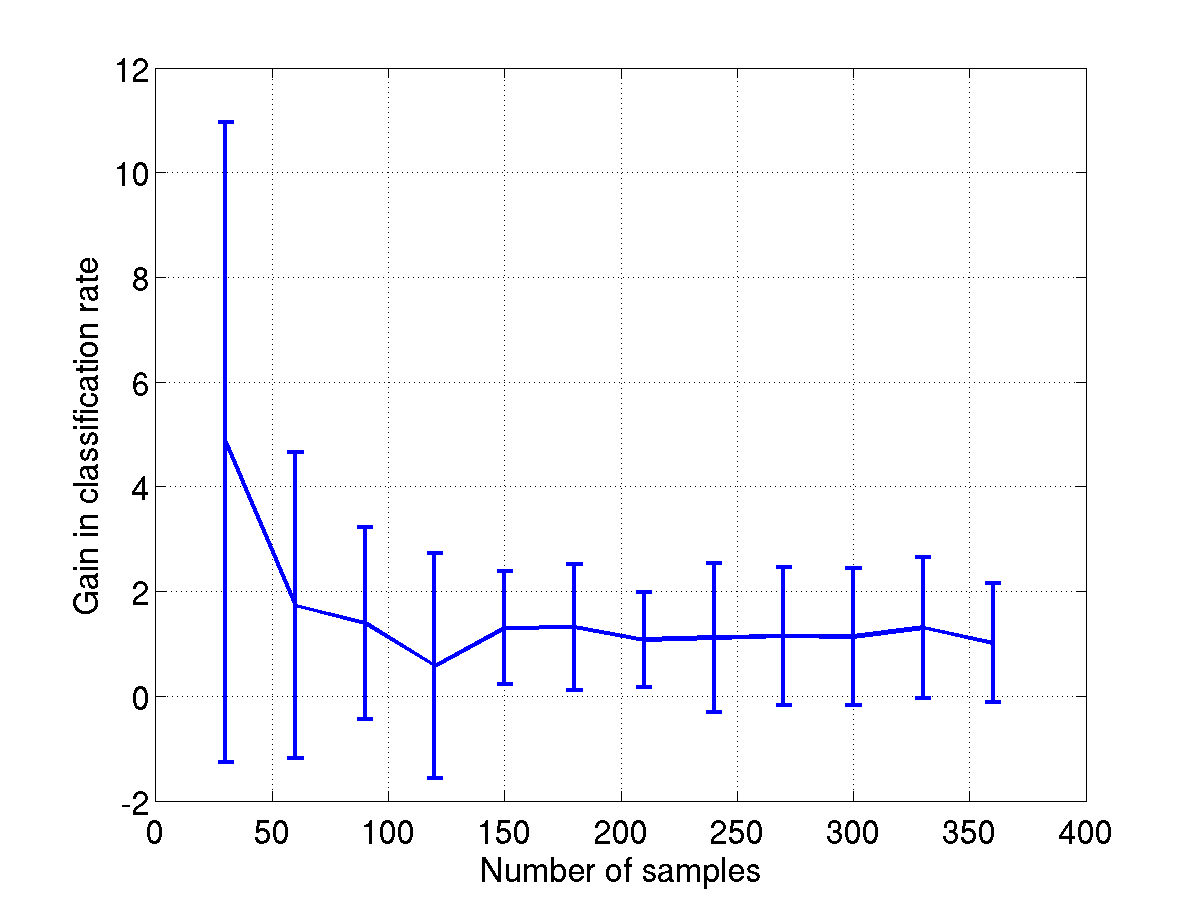
\includegraphics[width=0.95\linewidth]{figs/exp1}
  \caption{Classification results: Difference in performance between \emph{NoAdapt} and our method  on the
 classification of the grasp types.}
  \label{fig:diff_cla}
\end{figure}

\begin{figure*}[ht] \centering
  \begin{tabular}{cc}
    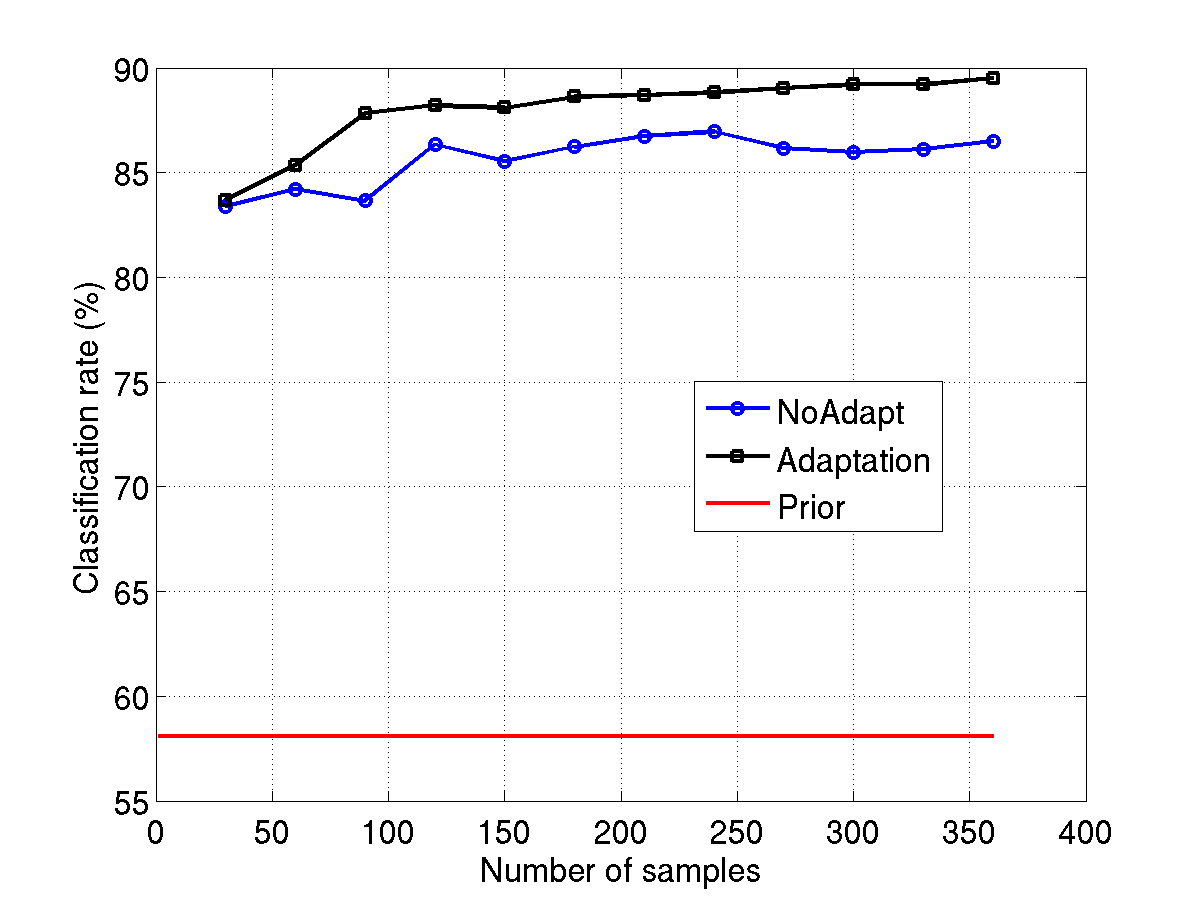
\includegraphics[width=0.45\textwidth]{figs/exp1_abs_best} &
    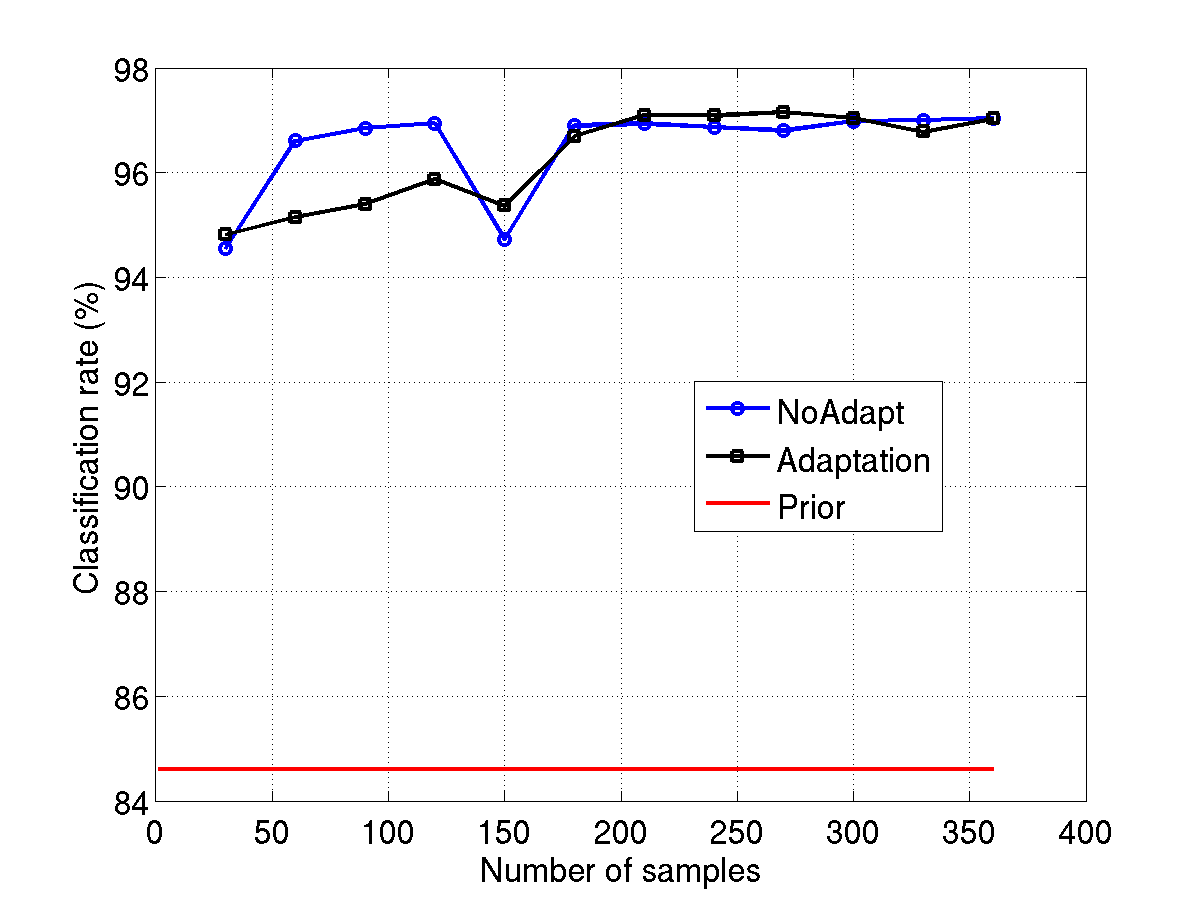
\includegraphics[width=0.45\textwidth]{figs/exp1_abs_worst} \\
    $(a)$ & $(b)$ \\
  \end{tabular}
  \caption{Classification results: $(a)$ Best classification rate gain of the adapted model compared to
 \emph{NoAdapt} and \emph{Prior} on a particular subject; $(b)$ worst performance on another subject.}
  \label{fig:cla_abs}
\end{figure*}

\begin{figure}[ht]
  \centering
  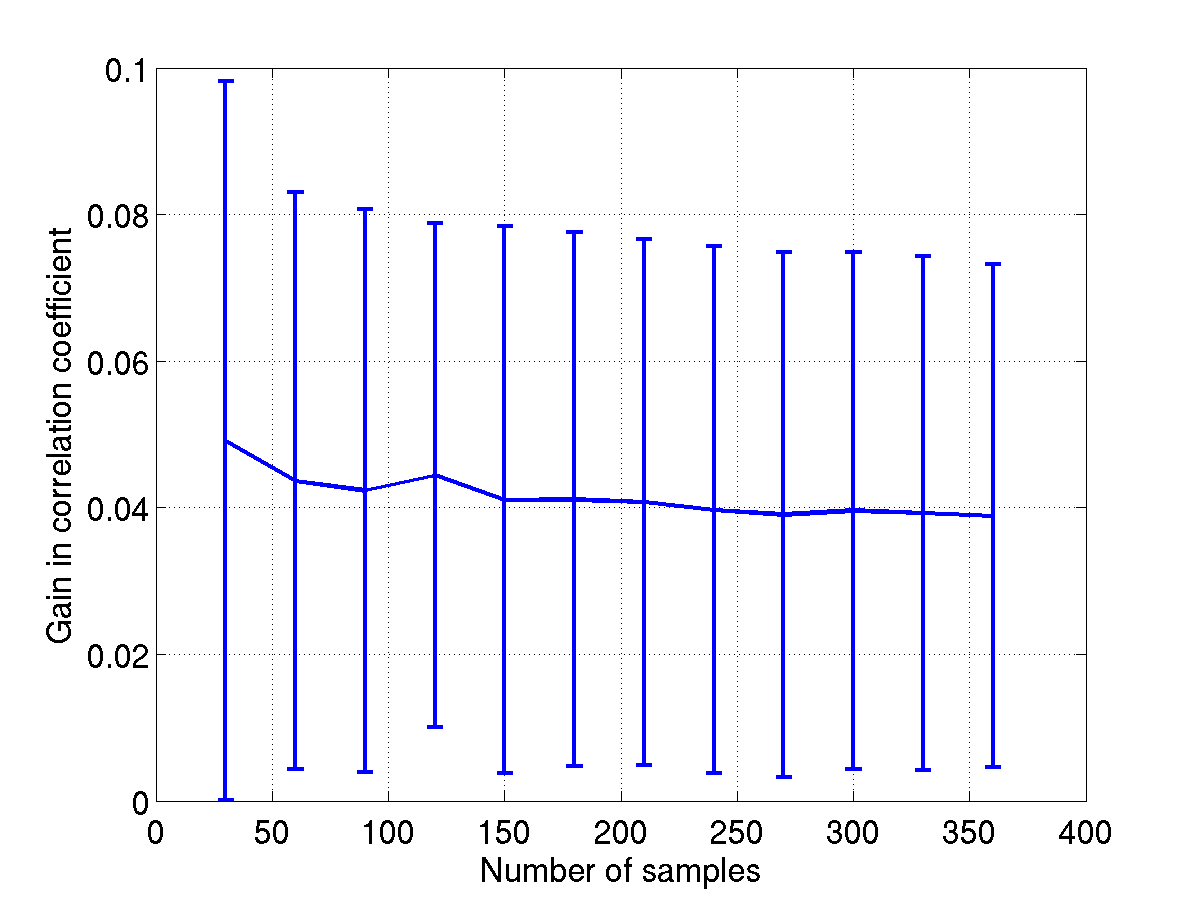
\includegraphics[width=0.95\linewidth]{figs/exp2}
  \caption{Regression experiments: Difference in performance between \emph{NoAdapt} and our method  on the
 regression of the force.}
  \label{fig:diff_reg}
\end{figure}

\begin{figure*}[ht] \centering
  \begin{tabular}{cc}
    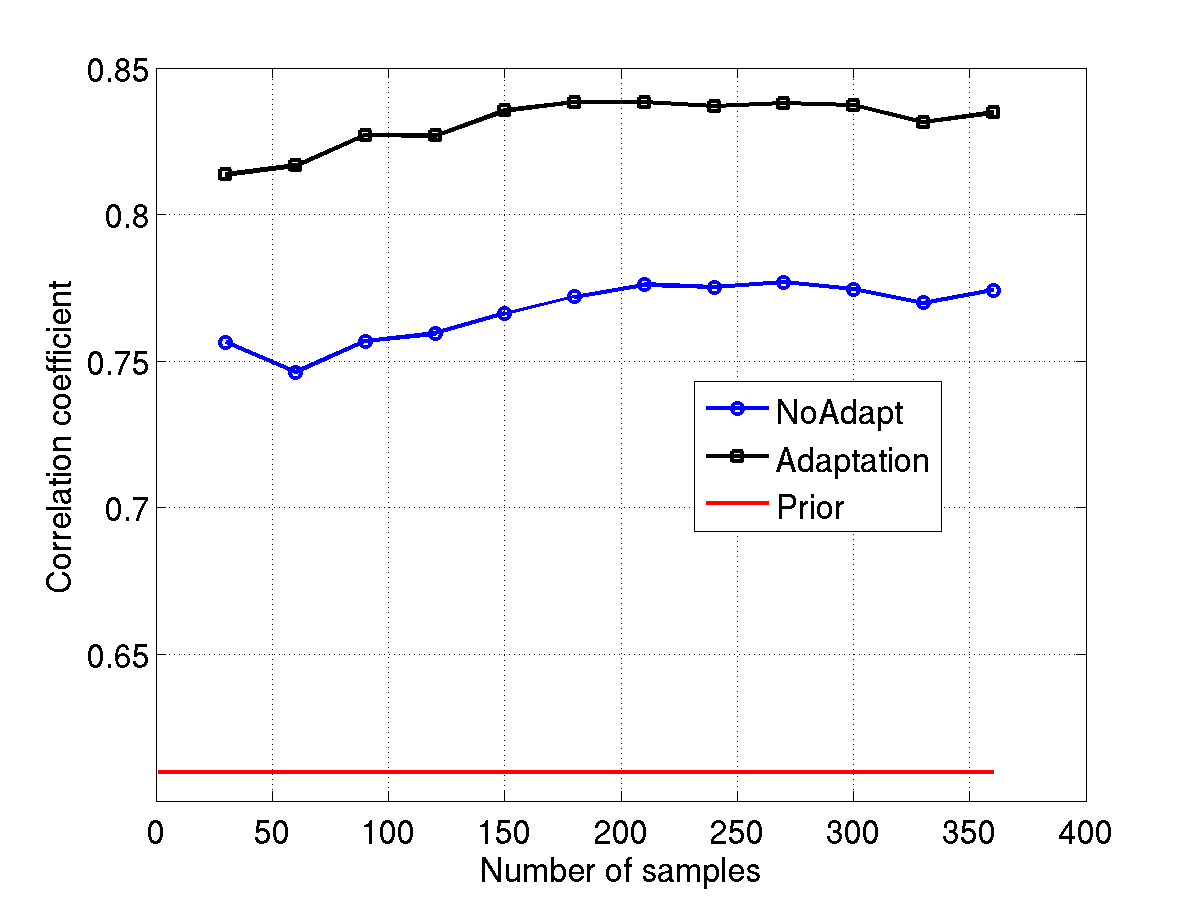
\includegraphics[width=0.45\textwidth]{figs/exp2_abs_best} &
    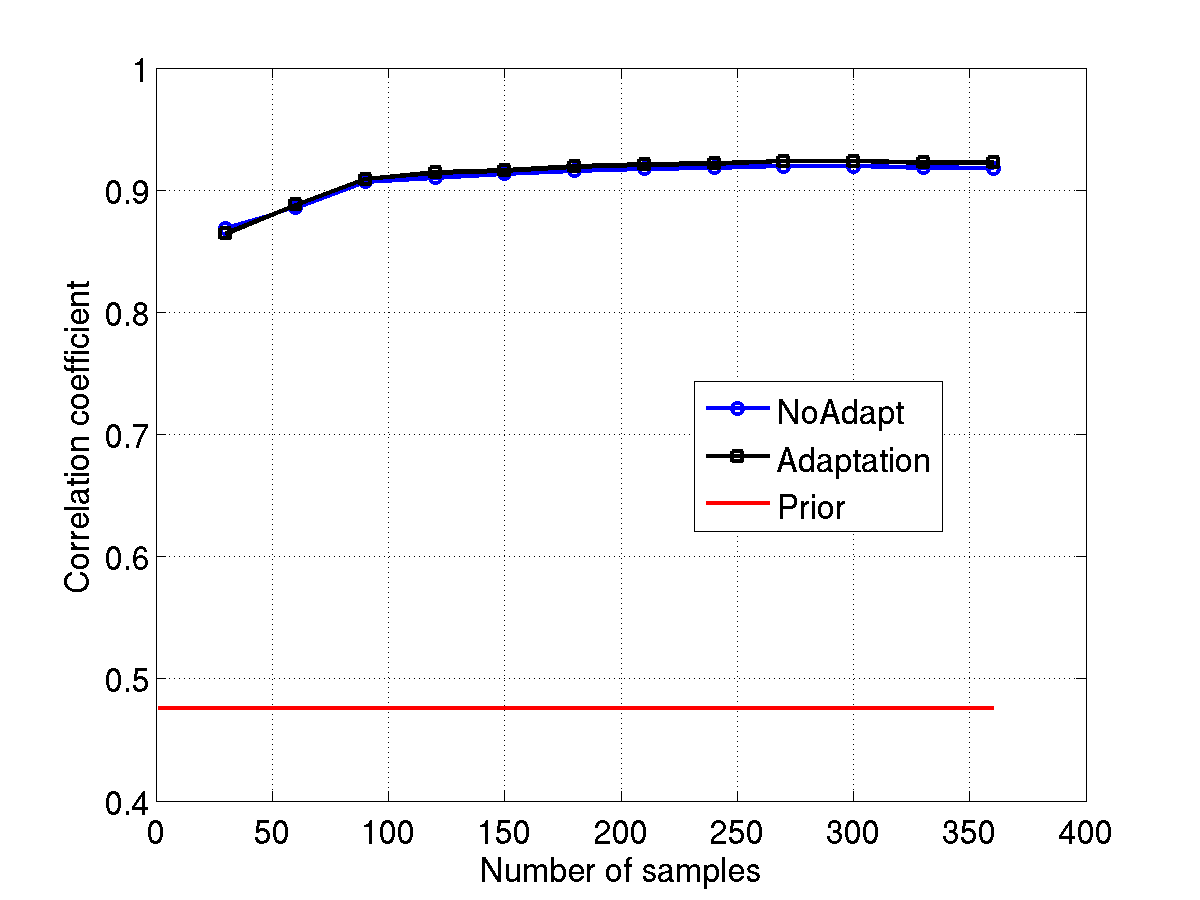
\includegraphics[width=0.45\textwidth]{figs/exp2_abs_worst} \\
    $(a)$ & $(b)$ \\
  \end{tabular}
  \caption{Regression experiments: $(a)$ Best correlation coefficient gain of the adapted model compared to \emph{NoAdapt}
 and \emph{Prior} on a particular subject; $(b)$ worst performance on another subject.}
  \label{fig:reg_abs}
\end{figure*}


\subsection{Grasp Classification}
\label{subsec:classification}
classification.


\subsection{EMG to Force Regression}
\label{subsec:regression}
regression.


\section{Conclusions}
\label{sec:conclusions}
The model adaptation method presented in this paper stems from a
problem in adaptive hand prosthetics, namely: is it possible to help a
patient to learn to use a dexterous hand prosthesis 
%in a quicker and
%better way, 
by exploiting the common features found in models trained upon other
patients?
The answer, at least as far as healthy subjects are concerned, is yes:
we have hereby presented a novel method for model adaptation in
machine learning, using Least-Squares SVMs; the idea is to build a SVM
solution which is \emph{close} to one of a set of pre-stored
models. The choice of which model to use among the pre-trained ones,
as well as the parameter $\beta$, determining the degree of closeness
to start the training from, are completely automatic, as we use an
estimation of the generalization error.

We tested our method on a database built with EMG and force data from
$10$ healthy subjects, trying to improve the training times and
asymptotic performance of one subject by pre-training on other
subjects. The outcome of the experiment is positive: our method gains
consistently both in the classification and regression tasks in the
best and average cases, and it resorts to the non-adaptive performance
in the worst.

Therefore, it is apparent that a large amount of knowledge stored in
LS-SVM models is common to all subjects, which is obviously due to the
analogies among the tasks performed by the subjects, as well as to the
anatomical similarities among the arms and the careful positioning of
the electrodes on the subjects' forearms. A further interesting point
is that, almost uniformly, models obtained by adaptation from a
pre-trained model obtain a \emph{better} performance than those
trained from scratch. This result is somehow surprising, although very
encouraging, and subject of future research.

Notice that we present no results on a real prosthetic/robotic hand so far --- this is subject of immediate-future research. We successfully applied a similar system to the DLR-II mechanical hand (see \cite{2008.ICRA,2008.BioCyb}), and since the accuracy of the system presented here is analogous to that of the one therein, there is no reason why the results presented here should not apply as well in the practical case. One interesting possibility is that of using this system to speed up the adaptation of an already existing dexterous hand prostheses, such as, e.g., Touch Bionics's i-LIMB \cite{ilimb} prosthetic hand, as already mentioned in the introduction.

Lastly, let us consider the fact that, most likely, the overall
performance of the method will increase when more subjects are
available, since this would mean a larger probability of finding a
matching pre-trained model. In a clinical setting, this means that
after an experimental phase, adaptive prostheses employing this method
could actually be built. It remains, of course, to discover whether
this idea can be transferred to amputees: amputations are, obviously,
non-controlled, traumatic events (except in some cases), and therefore
stumps exhibit much more variability than healthy forearms. This is
the subject of ongoing as well as future research.


\section*{Acknowledgments}

This work is partially supported by the project NEURObotics,
FP6-IST-001917.

{\small
\bibliographystyle{IEEEtran}
\bibliography{paper}
}

%% \begin{IEEEbiography}{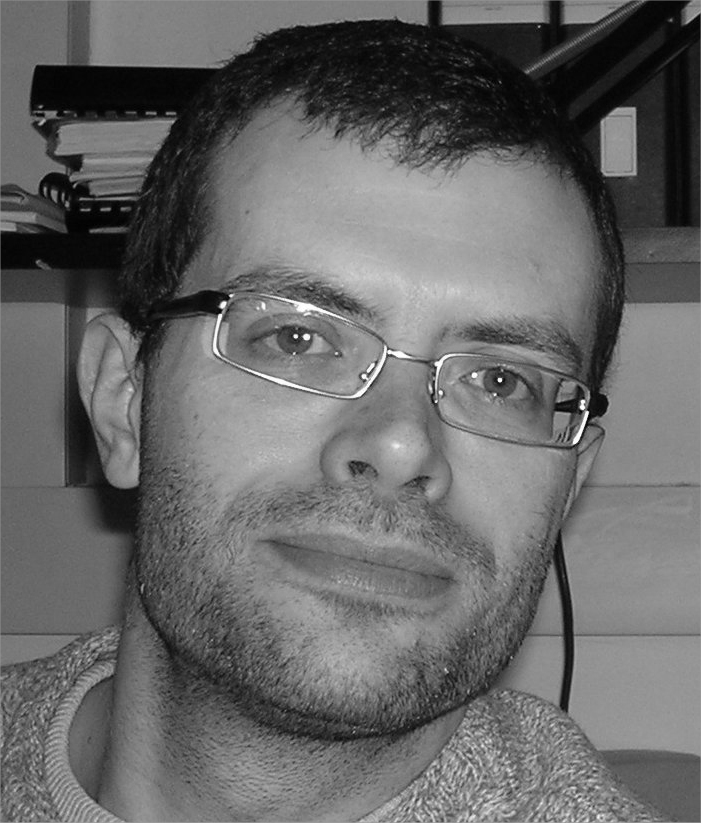
\includegraphics[width=1in,height=1.25in,clip,keepaspectratio]{claudio}}{Claudio Castellini}
%% biography
%% \end{IEEEbiography}

%% \begin{IEEEbiography}{\includegraphics[width=1in,height=1.25in,clip,keepaspectratio]{patrick}}{Patrick van der Smagt}
%% biography
%% \end{IEEEbiography}

%% \begin{IEEEbiography}{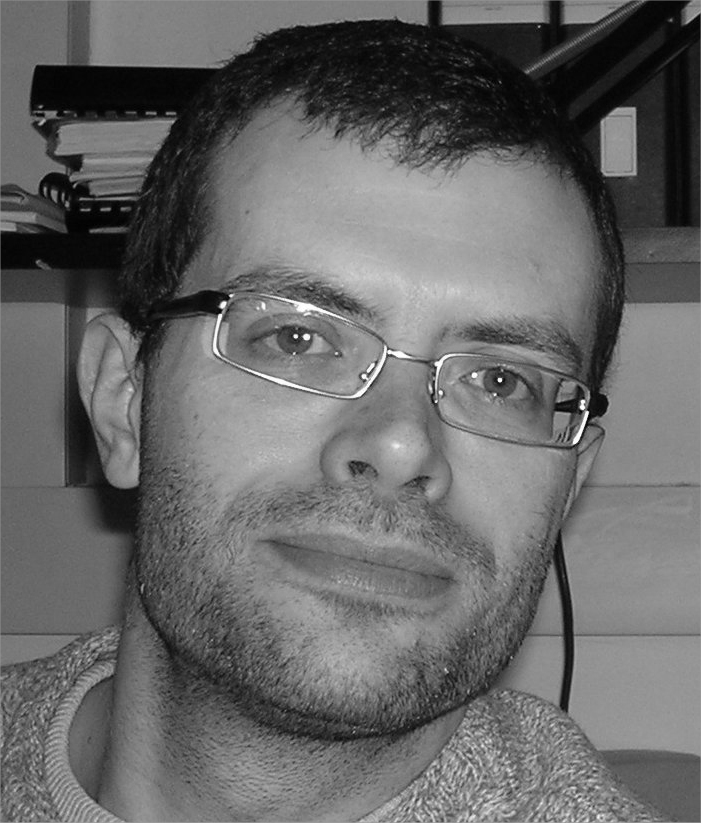
\includegraphics[width=1in,height=1.25in,clip,keepaspectratio]{claudio}}{Giulio Sandini}
%% biography
%% \end{IEEEbiography}

\end{document}
